\documentclass[12pt]{article}
\usepackage{multicol}
\usepackage[banglamainfont=BenSenHandwriting, banglattfont=Siyam Rupali, feature=0, changecounternumbering=0]{banglatex}
\usepackage[top=8em, left=10em, right=10em, bottom=8em]{geometry}
\usepackage{verbatim,spverbatim, hyperref, tcolorbox, hologo, enumerate, amsthm, xpatch, amsfonts, amssymb, amsmath, enumerate, chngcntr, pgffor}
\usepackage{tikz}
\usetikzlibrary{calendar,backgrounds,matrix}
\usepackage{fancyhdr}
\hypersetup{hidelinks=yes}
\tcbuselibrary{breakable}

\def\fileversion{v0.1}
\def\filedate{18 October, 2016}
\def\banglatex{\textsc{Bangla}\hologo{TeX}}
\newcommand{\pkn}[1]{\texttt{#1}}
\addto\captionsbengali{%
  \renewcommand{\contentsname}{Table of Contents}%
}

\makeatletter
%making the word ``proof'' in proof env. bold and adding a : after it.
\xpatchcmd{\proof}{\itshape}{\bfseries}{}{}
\xpatchcmd{\proof}{\@addpunct{.}}{\@addpunct{:}}{}{}
\linespread{1.1}
\def\@banglanumber#1{\expandafter\@@banglanumber\number#1\@nil}
\def\@@banglanumber#1{\ifx#1\@nil
  \else\char\numexpr#1+''09E6\relax\expandafter\@@banglanumber\fi}
\def\tobangla#1{\expandafter\@banglanumber\csname c@#1\endcsname}
\def\numtobangla#1{\@@banglanumber#1\@nil}\addto\captionsbengali{\renewcommand\proofname{\bfseries প্রমাণ}}
\newenvironment{solution}{\proof[\bfseries সমাধান]}{\endproof}

\newcommand{\callogo}{
  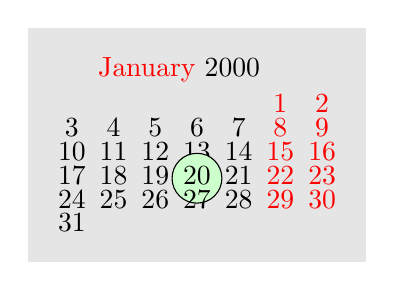
\begin{tikzpicture}[scale=1,every day/.style={anchor=mid},show background rectangle,
      background rectangle/.style={fill=gray!20!white}]
    \path (0,0)  node
          {\tikz \calendar[dates=2000-01-01 to 2000-01-31,week list,
              month label above centered,month text=\textcolor{red}{\%mt} \%y-,day yshift=2ex]
            if (Saturday) [red]
            if (Sunday) [red]
            if (equals=2000-01-20) {\draw[fill=green!20!white] (0,0) circle (9pt);};};
  \end{tikzpicture}
}

\begin{document}

\section*{সূচিপত্র }
\newpage

\subsection*{গোধুলি বেলা }
\hrule
\vspace{0.5in}
বলেছিলে আসবে।\\
সারাটা বিকাল বসেছিলাম তোমার অপেক্ষায়\\
জানালার পাশে ওই ধুলো ওড়া রাস্তাটার দিকে তাকিয়ে\\
এক এক সবাই চলেছে\\
এত ভীড়ের মাঝেও খুজেছিলাম তোমায়,\\
ধুলো ওড়ছিল ধোঁয়াশায় ঢেকে যাচ্ছিল আশাগুলো\\
পশ্চিমের কোলে লজ্জায় রাঙা সূর্যটাও ঢলে পড়ল\\
বাসায় ফিরল পাখিরা।।\\
হঠাত দেখি দুচোখ জলে ভরে এলো কান্নায়\\
ভেবেছিলাম প্রত্যেক বারের মত বুকে এসে জড়িয়ে নেবে\\
কিন্তু তুমি এলেনা,\\
রাতের গাঢ় আঁধারে হারিয়ে গেল স্বপ্নটা।।\\

\noindent
আজ আরও এক গোধুলি বেলা।\\
মনের কোনো এক কোণে আজ বাজছে তোমার গান,\\
সুরটা বোধ হয় মিশে যাচ্ছে সানাই এর সুরে\\
ভাষাটা কিন্তু আজও ভুলিনি, ভুলিনি সে চোখের জলের আবেদন\\
লাল বেনারসীতে সাজিয়েছি নিজেকে\\
আজও আছি পথের দিকে চেয়ে\\
যদি তুমি আসো...\\

\noindent
শুভদৃষ্টি হলো, তাকাতে পারিনি সে চোখে\\
পুরুত মশাই মন্ত্র বলতে আরম্ভ করলো\\
কানে আসছিল সেই বিদায় বেলার কথা--\\
``ফিরে আসব''\\
সবই কি ছিল মিথ্যে প্রহসন।।\\
রাঙা সিঁদুরে ভরিয়ে দিল সিঁথেটা\\
চোখ দুটো আবার কান্নায় ভিজেছিল কি?\\
ভিজেছিল বোধহয়,\\

\noindent
এক অজানা কষ্টে ভিতরটা আজ ছারখার\\
জানি আর তুমি আসবেনা\\
আর দেখবনা স্বপ্নটা।।   \\
\newpage

\subsection*{যন্ত্রণা }
\hrule
\vspace{1in}
তুমিতো জাননা, আমি জানি\\
কত যন্ত্রণা, লাঞ্চনা বুকে নিয়ে নিশ্চুপ হয়ে থাকি।\\
বুকের ভিতর জ্বলতে থাকা এক আগ্নেয়গিরির\\
খবর তো তুমি জাননা,\\
টগবগ করে ফুটতে থাকা তার রক্তাক্ত লাভার\\
গভীরতা তো তুমি জাননা।\\
আমি জানি, ধিক ধিক করে জ্বলা\\
সে আগুন বুকে চেপে দিন থেকে মাস,\\
সদর্পে, সগৌরবে বলি\\
এই তো সুখ ছুঁয়েছে আমার অধর\\
এই তো তার মাদকতায়\\
নিভেছে সেই অগ্নির লেলিহান শিখা\\
কত ঝড়, কতো হাহাকার বুকে নিয়ে নিশ্চুপ হয়ে থাকি\\
বুকের ভিতর বাজতে থাকা এক দামামার খবর তুমি জাননা\\
কেমন তার আঘাতে কেঁপে ওঠে স্বপ্নের ভীতটা\\
গুপ্তধনের আশায় সেই ধ্বংসস্তুপ আগলে রাখি\\
তুমিতো জাননা, আমি জানি\\
কত না পাওয়া, না থাকা বুকে নিয়ে নিশ্চুপ হয়ে থাকি। \\
\newpage

\subsection*{তুমি আসবে বলেই }
\hrule
\vspace{1in}
আমি ছোঁবনা বাইরের ওই কোলাহল\\
ওই কোলাহল কখনো ছোঁবেনা আমাকে\\
আমি দেখবনা ওই জমে থাকা ভীড়\\
ওই ভীড় দেখবেনা আমাকে\\
তবু বসে আছি জানালার পর্দাটা টেনে\\
কত সহস্র যোজন পথ পেরিয়ে আসবে সে\\
বলবে ``ভয় কি? মিশে যাও আমার রন্ধ্রে রন্ধ্রে\\
চল পা রাখি ওই রাস্তাটায়''\\
লুকাব নিজেকে তার আড়ালে\\
বেরিয়ে পড়ব নতুন এক পৃথিবীর খোঁজে\\
মানুষের মত দেখতে এই প্রাণীগুলোর ভীড় ছাড়িয়ে\\
যাব সেই আনন্দ উদ্যানে, পাব মুক্তির আস্বাদ\\
বুকের ভিতর কোকিয়ে ওঠা সত্বাটা আবার হাসবে\\
মন পাখিটা আবার পাখা মেলাবে\\
ওই দিগন্ত ছোঁয়া অসীম নভোনীলে\\
আবার একটু নিশ্বাস নেবে\\
আজও বসে আছি জানালার পর্দাটা টেনে।।\\
\newpage

\subsection*{ও শ্যাম }
\hrule
\vspace{1in}
ও শ্যাম, লাজ রাখি? না তোমায় রাখি?\\
বরং আমার সকল দিয়ে তোমায় রাখি\\
ও শ্যাম, লাজ রাখি? না তোমায় রাখি?\\

\noindent
তবে ওরা যে বলে কলঙ্কিনী?\\
বয়েই গেছে, আমিতো শুধু তোমায় চিনি\\
তোমায় জানি, তোমায় মানি\\
হইনা তবে কলঙ্কিনী।\\

\noindent
অহংকারী না কি অভিমানী?\\
যা বলে ছাই বলুক ওরা\\
আমি তোমার গর্বেই গরবিনী\\
রাগ জমাবো? নাকি গান শোনাব?\\
তার চেয়ে শ্যাম তোমার হব!\\

\noindent
চুল বাঁধব মালতী ফুল খোঁপায় পরি\\
শাড়ি হবে বালুচরী আর গলায় হার সাতনরী\\
নষ্ট বলে বলুক লোকে\\
আমিতো তখন রাইকিশোরী!\\

\noindent
কলঙ্ক না আদর মাখি?\\
ও শ্যাম, আমি বরং তোমায় রাখি।।\\

--৫/১১/১৫
\newpage

\subsection*{যদি কথা দাও}
\hrule
\vspace{1in}
যদি কথা দাও বিচ্ছেদের তিরে বিঁধবেনা\\
তবে হতে রাজী আছি কানায় কানায় উপচে পরা এক নদী\\
তোমার বুকের অতলে প্রতি স্পন্দনে বইব চঞ্চল গতি\\
ভেজাবো তোমায় মর্মে মর্মে অনন্ত কাল নিরবধি।।\\

\noindent
যদি কথা দাও তুমি ভিজবে আমাতে\\
তবে আমার যত দীনতা হীনতা এখনই কাটিয়ে উঠি\\
শিরাতে ধমনীতে, দিবাতে নিশিতে ছড়াই তোমার উপস্থিতি\\
আমার সকল বারতা ফুটুক হয়ে বর্ষার নিপবীথি।।\\

\noindent
যদি বল চৈত্রের শেষ বিকেলে সূর্যের সাথে ঢলবেনা\\
তবে কুসুমে কাননে বসন্তের সুর হয়ে বাজি\\
কৃষ্ণচুড়ার আবির মেখে, বৈশাখী মেঘের কাজল মোহময়ী রূপে সাজি।।\\

\noindent
যদি বল হারাবেনা ওই জমে ওঠা ভীড়ে\\
তবে আরও একবার ফিরে যাই ওই শৈশবে\\
কুড়িয়ে নিই একমুঠো সরলতা, খুঁজে আনি নিষ্পাপ সেই হাসি\\
সব বাঁধন ছাড়িয়ে হই সেই স্রোতস্বিনী বানভাসী।\\

\noindent
যদি দাও কথা জ্বালাবেনা ওই ক্রোধানলের চিতায়\\
তবে আর একটু নিঃশ্বাস চুরি করে\\
তোমাতে নিজেকে উজার করে আর একটুখানি বাঁচি।।\\

--৯/৫/২০১৬
\newpage

\subsection*{চলে এসো }
\hrule
\vspace{1in}
যখন তারার আলো লজ্জায় মুখ ঢাকে\\
চলে এসো সেই মন খারাপের রাতে\\
সেই ভীষণ কঠিন বজ্রসম আঘাত\\
সেই ভীষণ ঝড়ের গভীর কালো রাত\\
আমার ভাঙ্গা ঘরে প্রদীপখানি জ্বেলে\\
ছিন্ন আঁচল আড়াল করে থাকব বসে\\
দুয়ার খানি রাখব খুলে সেই উত্তাল বরষাতে\\
চলে এসো সেই মন খারাপের রাতে।\\

\noindent
যখন তুমি নিঃস্ব আবার, রিক্ত আবার\\
জীবন নদী স্রোত হারিয়ে স্তব্ধ আবার\\
বৃষ্টি হয়ে নামব আমি তোমার পরে\\
মেঘ মল্লার বাঁধব তোমার ছিন্ন বীণার তারে\\
থাকব বসে আঁচল খানি পেতে\\
চলে এসো সেই মন খারাপের রাতে।\\

\noindent
দুঃখ যখন ছোঁবে তোমায়\\
যখন আশার আলো অন্ধকারে মুখ লুকায়\\
বুকে তোমার লুকিয়ে নিয়ে থাকব পাহারাতে\\
এস আমার দ্বারে, সেই মন খারাপের রাতে।।\\
\newpage

\subsection*{মৃত্যুছায়া }
\hrule
\vspace{1in}
রোজ রাতে হাতছানি দেয় মৃত্যুর ওই করাল গ্রাস\\
আঁতকে উঠি নিঃস্ব হয়ে ঘামে ভেজা অন্তর্বাস\\
হাত বাড়াই ছোঁব বলে তোর ভালবাসার উষ্ণতা\\
নিরুত্তাপ তোর্ স্বাসপ্রশ্বাস জানায় আমার প্রেমের ব্যর্থতা\\
রাজনীতি থাবা বসায় হৃতপিন্ডের কোণায় কোণায়\\
ধুকপুকুনি চায় বন্ধ হতে, প্রতিশ্রুতি মিথ্যা শোনায়\\

\noindent
অন্ধকার ছোবল মারে বিষিয়ে দেয় অন্তনীর\\
শকুনগুলো ছিঁড়ে খায় স্বপ্নের ওই নীল্ শরীর। \\
\newpage

\subsection*{স্বপ্নময়}
\hrule
\vspace{1in}
তোমার পাঁচমিশলি রঙে চোখ ধাঁধিয়ে গেল\\
এক ঝটিকায় বিধ্বস্ত আমার স্বপ্নলোক\\
স্বপ্নময়, কোথায় তুমি? কোনটা তোমার রঙ?\\
প্রথমবার বললে তুমি ``রাখ তোমার ওসব ঢঙ''।।\\

\noindent
স্বপ্নময়, তুমিই কি সে?\\
যার তীব্র প্রেমের আগুন একদা জ্বালিয়েছিল আমাকে?\\
বল, তুমিই কি সে?\\
\newpage

\subsection*{অভিনয়}
\hrule
\vspace{1in}
বুকের মাঝে থেকে থাকা একটা দীর্ঘশ্বাস\\
তোমার আমার মাঝে অযাচিত এক রাজনীতি\\
আঘাতের পর আঘাত ভেঙ্গে পড়া পাঁজরের কত হাড়\\
আর মনের কোণে জমে থাকা একরাশ হতাশা\\
চোখের কোণে এসে থেমে থাকা কান্না\\
হাসির আড়ালে লুকানো যন্ত্রণা\\
আবিষ্কারের অপেক্ষায়।\\

\noindent
মুখরতার রঙ্গে মাখা মৌনতা\\
ছিন্ন বস্ত্র জড়িয়ে লাজ ঢাকার বৃথা প্রয়াস\\
পবিত্র প্রেমের কন্ঠ আজ অভিনয়ে রুদ্ধ\\
এ যেন কি এক অদ্ভূত পরিহাস।\\
ঘর বাঁচাতে ঘরের ভিতর লুকোচুরির খেলা,\\
খেলতে খেলতে হারিয়ে যাওয়া খুঁজে নেওয়ার আশায়।।\\

-২৫.৩.২০১৬
\newpage

\subsection*{ভালবাসার উপহার }
\hrule
\vspace{1in}
ভালবাসা উপহার দিল সুখ\\
ভালবাসা উপহার দিল তোমার আমার\\
সৃষ্টি করা এক নতুন ইতিহাস\\
জোয়ার লাগে আবার শান্ত দেহে\\
কানায় কানায় উপচে পড়া\\
উত্তাল সেই ঢেউ\\
সে সাগরে সাঁতরে বেড়াও\\
উষ্ণ বুকের উথাল পাথাল\\
বৃন্তজোড়া আঁকড়ে ধরে\\
সুখ সাগরে মিষ্টি নেশায়\\
হাতরে বেড়াও\\
আঁচড় কামড় আঁকড়ে ধরা\\
স্বর্গীয় সেই রসের ধারা\\
স্তন্যযুগল আদরে মেখে রক্তজবা\\
আবেশ আবেশ গন্ধে মাখা\\
ক্লান্ত রাতের আদুল ভিজে দেহ\\
টুকরো টুকরো বিছিয়ে দিয়ে\\
বক্ষ মাঝে যুগল শয়ন। \\
\newpage


\subsection*{শেষ চাওয়া }
\hrule
\vspace{1in}
নাইবা দিলে মনে ঠাঁই\\
নাইবা দিলে ভালবাসা\\
তবু মনে রাখতে চাই\\
নিরাশাতেও একটু আশা\\
যদি তুমি নাইবা এলে\\
এ শূন্য দ্বারে ওগো প্রিয়\\
আশীষ না হয় নাইবা দিলে\\
অভিশাপেই, মন ভরিয়ো\\
আমার যদি নাইবা হলে\\
অন্য কারোর হয়েই থেকো\\
জড়িয়ে বুকে নাইবা নিলে\\
চারণ তলেই ফেলে রেখো\\
স্বপ্ন যদি নাইবা দিলে\\
আঁখিপাতে শ্রাবণ দিও\\
মোর অশ্রুনদীর অশ্রুজলে\\
শুধু একটি বার গা ভাসিয়ে\\
নেই গো আমার দেওয়ার কিছু\\
নেই গো কিছু পাওয়ার\\
দিও শুধু একটু সময়\\
তোমার পানে চাওয়ার\\
ধন্য হবে জীবন আমার\\
ধন্য হবে মরণ\\
সুখে না হয় নাইবা নিলে\\
যদি দুঃখেও কর স্মরণ।।\\
\newpage

\subsection*{নারী }
\hrule
\vspace{1in}
``মা তুমি রাঁধতে পার?''\\
``পঞ্চব্যঞ্জন, নবরত্ন, বিরিয়ানি শুক্ত পোলাও?''\\
``আল্পনাটা দিতে পারো ?''\\
পারলে তুমি লক্ষী মেয়ে, আর না পারলে?\\
'কুলক্ষণী', 'অকল্যাণী'-র তকমা জোটে।।\\
পারবনা ওই ঘুণধরা মাপকাঠিতে নিজেকে মাপতে।\\
ওই ছকে বাঁধা ঘোমটা দেওয়া জীবন আগলে বাঁচতে।\\
তারচেয়ে যদি হই দুর্ধর্ষ কোনো আকাশচারী?\\
তপ্ত মরুপথের নির্ভয় কোনো ঘোড়সওয়ারী?\\
ক্ষতি হবে? যদি এক ডুবেতে কুড়িয়ে আনি মুক্ত-ঝিনুক,\\
যদি হই সপ্তসিন্ধূ জয়ী কোনো এক সাঁতারু?\\
``বাঃ! মা তুমি তো বেশ সাহসী!''\\
--করবেন তবে কুলবধূ?\\
যদি বলি পারবনা স্বামীর জন্য পাশাখেলার পণ্য হতে\\
পারবনা অগ্নি পরীক্ষায় সতীত্বের প্রমাণ দিতে\\
পারবনা নৃত্য গীতে তুষ্ট করে স্বামীর প্রাণ ফেরাতে\\
কোথায় সেই প্রসংসা তো আর শুনিনা?\\
কোথায় সেই গদগদ হাসি আর দেখিনা।\\
``যা দেবী সর্ব ভূতেষু মাতৃরুপেণ সংস্হিতা''\\
আরও একবার অনুরণিত হোক এই মাতৃবন্দনা\\
শঙ্খধ্বনি, কাঁসর, ঘন্টায় আবির্ভূত হও দেবী চন্ডিকা\\
নিষ্প্রাণ কোনো মূর্তিতে না, সশরীরে এস নেমে\\
খড়গ, ত্রিশূল, বজ্র হাতে আন সেই বিপ্লব।।\\
বাঁচতে শেখাও লতিয়ে চলা এই প্রাণীটিকে।\\
নারী, তুমিই তোমার সহায়, তুমিই তোমার অবলম্বন।।\\
\newpage

\subsection*{প্রেম }
\hrule
\vspace{1in}
অপেক্ষাটা আজ শেষ হল\\
হঠাত দেখি এক ঝোড়ো হওয়া এসে ছুয়ে গেল আমায়,\\
কোমরের অববাহিকা বেয়ে সে উঠে এলো,\\
মিশে গেল রন্ধ্রে রন্ধ্রে।\\
তাকে অনুভব করলাম স্বপ্নে, ভালবাসায়, উদাসীনতায়,\\
নির্লজ্জের মত নিজেকে উজার করে দিলাম তার কাছে\\
অগাধ বিশ্বাসে।\\
সে এক পাগল হাওয়া, সে আজও অধরা,\\
বাহুমূলে জড়িয়ে চুম্বনে, বন্ধনে বাঁধলো আমায়\\
সে ঠোঁটের ছোঁয়া এখনো উষ্ণ, এখনো জীবন্ত।\\
হঠাত দেখি এলো চুলে তার লুকোচুরি\\
যত্ন করে লুকিয়ে রাখা তিলটাতে তার দুষ্টুমি\\
সে এক বাঁধন হারা মাতাল হওয়া।\\
সে ভাসিয়ে নিয়ে চললো আমায়\\
সে আমার বড়ই আপন, বড়ই কাছের উদাস হওয়া।।\\
\newpage

\subsection*{অভিমান }
\hrule
\vspace{1in}
ফিরিয়ে নাও কবি এ গান,\\
চাইনা অত প্রসংসা মাধুরী;\\
শরীর জুড়ে চাইনা শুধু মন\\
থাকুক কিছুটা হাড় মাংস ও\\
আর কিছুটা অবহেলা প্রত্যাখান।\\
দুর্ভাগ্যের পায়ে চুমু খেয়ে যেন বলতে পারি\\
``এই তো জীবন''।\\
যে ছিল অধরা সে অধরাই থেকে যাক\\
মনের চোরাগলিতে কান্নার মশাল জ্বেলে\\
খুজতে চাইনা তাকে।\\
রোদ্দুর যদি গা জ্বালিয়ে দেয়,\\
যদি কখনো চাঁদের শীতল আলোর জন্য মনটা কেঁদে ওঠে\\
ছুটে যাবনা সেই স্নিগ্ধ ছাওয়ায় প্রাণ জুড়াতে,\\
তার চেয়ে ঘরের কনে জ্বালিয়ে নেব এক প্রদীপ।\\
এত দ্বিধা-সংকোচে  যদি সে চায় হতে পলাতক\\
আটকাতে চাই না তাকে, বরং তার খামখেয়ালীর রঙে\\
তুলি ভিজিয়ে ঠোঁটে আঁকব হাসির রেখা।\\
চোখের তলায় কালি, উসকখুসকো অবিন্যস্ত চুল,\\
আলুথালু বেশ আর ছন্নছাড়া জীবন নিয়ে\\
আর দাঁড়াবনা তার সিংহদুয়ারে দরজা খোলার আশায়।\\
যা কিছু আমার অশুভ, সবটা কুড়িয়ে নিলাম।\\
পরিচিত শেয়াল, কুকুর, শকুনদের ভীড়ে হলাম নিরুদ্দেশ।।\\
\newpage

\subsection*{হংসমিথুন }
\hrule
\vspace{1in}
লাল পাহাড়ীর মেঠো পথে মোহনীয়া বন্ধুরে\\
বাজাও তোমার মোহন বাঁশি পূর্ণিমা সন্ধ্যেতে।\\
শালপিয়ালের স্নিগ্ধ ছাওয়ায়\\
ঝিমধরানো মাতাল হাওয়ায়\\
আমরা হব হংসমিথুন।।\\

\noindent
ময়ুরাক্ষীর বালুচরে, দেহযুগল বিছিয়ে দিয়ে\\
মুগ্ধ হয়ে শুনব বাঁশি।\\
সে সুর আমার অঙ্গে লেগে মন বীণাটা উঠবে বেজে\\
এলোমেলো ছন্দেতে,\\
চাঁদের আলোয় গা ভিজিয়ে\\
তোমার আলতো ছোয়ার আদর মেখে\\
নতুন রূপে উঠব জেগে\\
একরাতেতেই কাটিয়ে দিয়ে একশোটা জীবন।।\\
\newpage

\subsection*{বৃষ্টি }
\hrule
\vspace{1in}
বৃষ্টি তুই শপথ নিলি ঝমঝমিয়ে নামার\\
বৃষ্টি তুই জানিস তুই আমার, শুধুই আমার।\\
বৃষ্টি তুই অঝর ধারায়\\
তাই বুঝি বা মনটা হারায়\\
তপ্ত হৃদয় জড়িয়ে জ্বালা\\
গাঁথবে আবার গানের মালা।\\
সঙ্গে নেব বৃষ্টি তোকে\\
আমার প্রাণের দোসর সুখে দুখে,\\
মন চাষীরা ক্লান্ত যখন\\
মেঘের ভেলায় ভাসবি তখন\\
ঝিরঝিরিয়ে নামবি আবার\\
ভিজিয়ে দিয়ে মনের খামার।\\
আবার তাতে বীজ বুনবো\\
ভালবাসার গান বাঁধবো\\
মেঘলা জীবন মাতবে নেশায়\\
মাতাল হব নতুন আশায়।\\
মনে পড়ে রাত দুপুরে?\\
বাঁধন গুলো ছিন্ন করে\\
বুকে এসে ঝাঁপিয়েচিলাম?\\
বৃষ্টি আমি তোকেই প্রথম ভালোবেসেছিলাম।।\\
\newpage

\subsection*{হঠাৎ }
\hrule
\vspace{1in}
হঠাত যেদিন তোমায় দেখি\\
এই হৃদয় মাঝে কোনো\\
অনুভূতির সঞ্চার হয়নি,\\
শুধুই ভালোলেগেছিল তোমায়।\\

\noindent
হঠাত যখন তোমায় ভাবি\\
এই মনের মাঝে কোনো\\
আবেগের সঞ্চার হয়নি\\
শুধুই ভেবেছিলাম তোমায়।\\

\noindent
হঠাত যখন তুমি কাছে এলে\\
দুরু দুরু বুকে দাঁড়িয়েছিলাম\\
এই দুহাত তোমায় জড়িয়ে ধরেনি\\
শুধুই দুচোখ ভরে দেখেছিলাম তোমায়।\\

\noindent
হঠাত যেদিন তুমি দূরে সরে গেলে\\
এই ঠুনকো হৃদয় ভেঙ্গে যায়নি\\
শুধুই কাঁদিয়েছিলে তুমি আমায়।\\

\noindent
হঠাত করে যখন হাতটা ধরলে এসে\\
চলতে শুরু করেছিলাম অজানার খোঁজে\\
কোনো ঠিকানা দরকার হয়নি\\
শুধুই বিশ্বাস করেছিলাম তোমায়।।\\

--১৮/১১/২০১৫
\newpage

\subsection*{মনে পড়ে ? }
\hrule
\vspace{1in}
স্বপ্নময়, মনে পড়ে সেই বনলতাকে ?\\
সবুজের কোলে এলোকেশী, পাগলিনী।\\
ফিরিছিল আপন খেয়ালে,\\
হঠাত তার পথ আগলে দাঁড়ালে পথিকসম\\
দিব্যকান্তি, দীপ্ত দুই চোখ ঝলসে দিল তাকে\\
কঠিন বাস্তবকে উপেক্ষা করে আঁকড়ে ধরেছিল তোমায়\\
শ্যেনদের তীক্ষ্ণ দৃষ্টি এড়িয়ে\\
যাকে দিয়েছিলে নারীত্বের সম্মান\\
সেই বনলতা।\\

\noindent
বল মনে পড়ে ?\\
অবুঝ দুপুর, ক্লান্ত মন\\
অশেষ আকাশ, অসীম স্বপন\\
তার পর্ণ কুঠির ঘিরে আজও তোমার উপস্থিতি\\
কত আলো-আঁধারি, কত ঝড় ঝন্ঝা\\
কত শত কাঁটা-ঝাড় পেরিয়ে\\
আজ সে অনেক দূরে ইতিহাস হওয়ার অপেক্ষায়\\
হয়ত স্মৃতির পাতায় কোনো এক মন খারাপের রাতে\\
সে আবার ভেসে উঠবে\\
ঝাপসা চোখে পেতে চাইবে তার ছোঁয়া।\\
আকাশের কোলে এক কোণে তাকিয়ে দেখো\\
মিটি মিটি হাসছে তোমার সেই বনলতা।।

\newpage
\vspace{4in}
\begin{center}
  \textcolor{magenta}{\Huge সমাপ্ত}
\end{center}
\end{document}

  

